\section{Especificação}

% ------ estrutura

\subsection{Requisitos}
    \begin{frame}\frametitle{Requisitos Funcionais}
	Foram levantados os seguintes requisitos funcionais:
		\begin{itemize}
			\item Ferramentas de blocagem e borramento
			\item Ferramenta de simulação de \emph{streaming}
			\item Sessões de avaliação subjetiva
			\item Implementação de métricas objetivas
			\item Exibir vídeos
			\item Exibir resultados de avaliações
		\end{itemize}
    \end{frame}
    
\subsection{Arquitetura}
    \begin{frame}\frametitle{Módulos do sistema}
	O sistema é dividido em 4 módulos:
		\begin{itemize}
			\item Modelo (\emph{model})
			\item Serviço (\emph{service})
			\item Ferramentas
			\item Interface gráfica
		\end{itemize}
    \end{frame}
    
	\begin{frame}\frametitle{Visão geral}
		\begin{figure}
			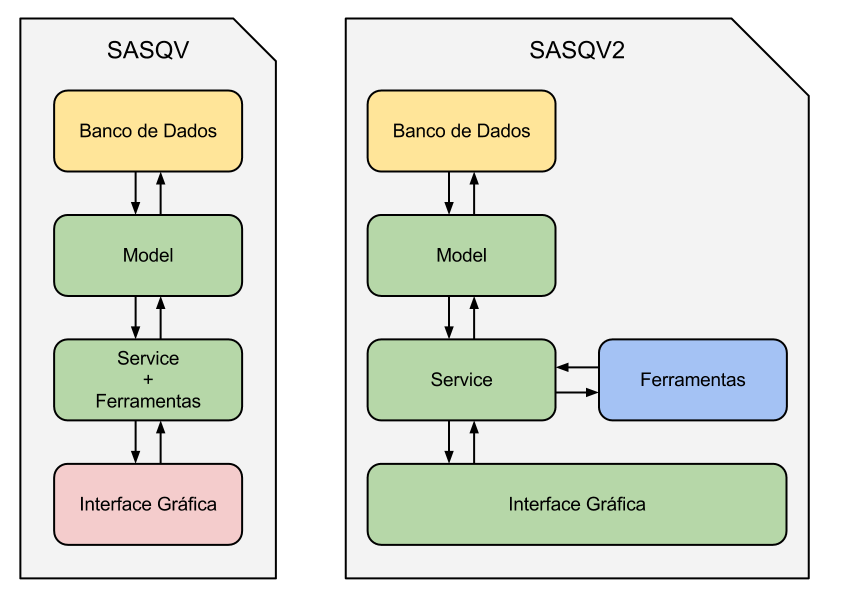
\includegraphics[width=0.8\textwidth]{./imgs/arquitetura.png}
			\caption{Representação geral do sistema}
			\tiny
			Fonte: Autoria própria.
		\end{figure}
	\end{frame}
